\begin{flushleft}
\doublespacing
I analysedelen har vi identificeret use-cases (se afsnit 5.1-5.3), opstillet domænet for Matador (se afsnit 5.4) og illustreret et systemsekvensdiagram over Matadorspillets overordnede sekvenser (se afsnit 5.5).
\subsection{Use-case diagram}
Use-case diagrammet viser en oversigt over vores samlede use-cases (se Figure \ref{use-case diagram}). Det ses her, at en Player kan Play Matador og Initialize Game. De resterende use-cases har et include relation til Play Matador, da disse er en del af use-casen at spille Matador, hvorimod Create Player er en del af Initialize Game.
\begin{figure}[H]
    \centering
    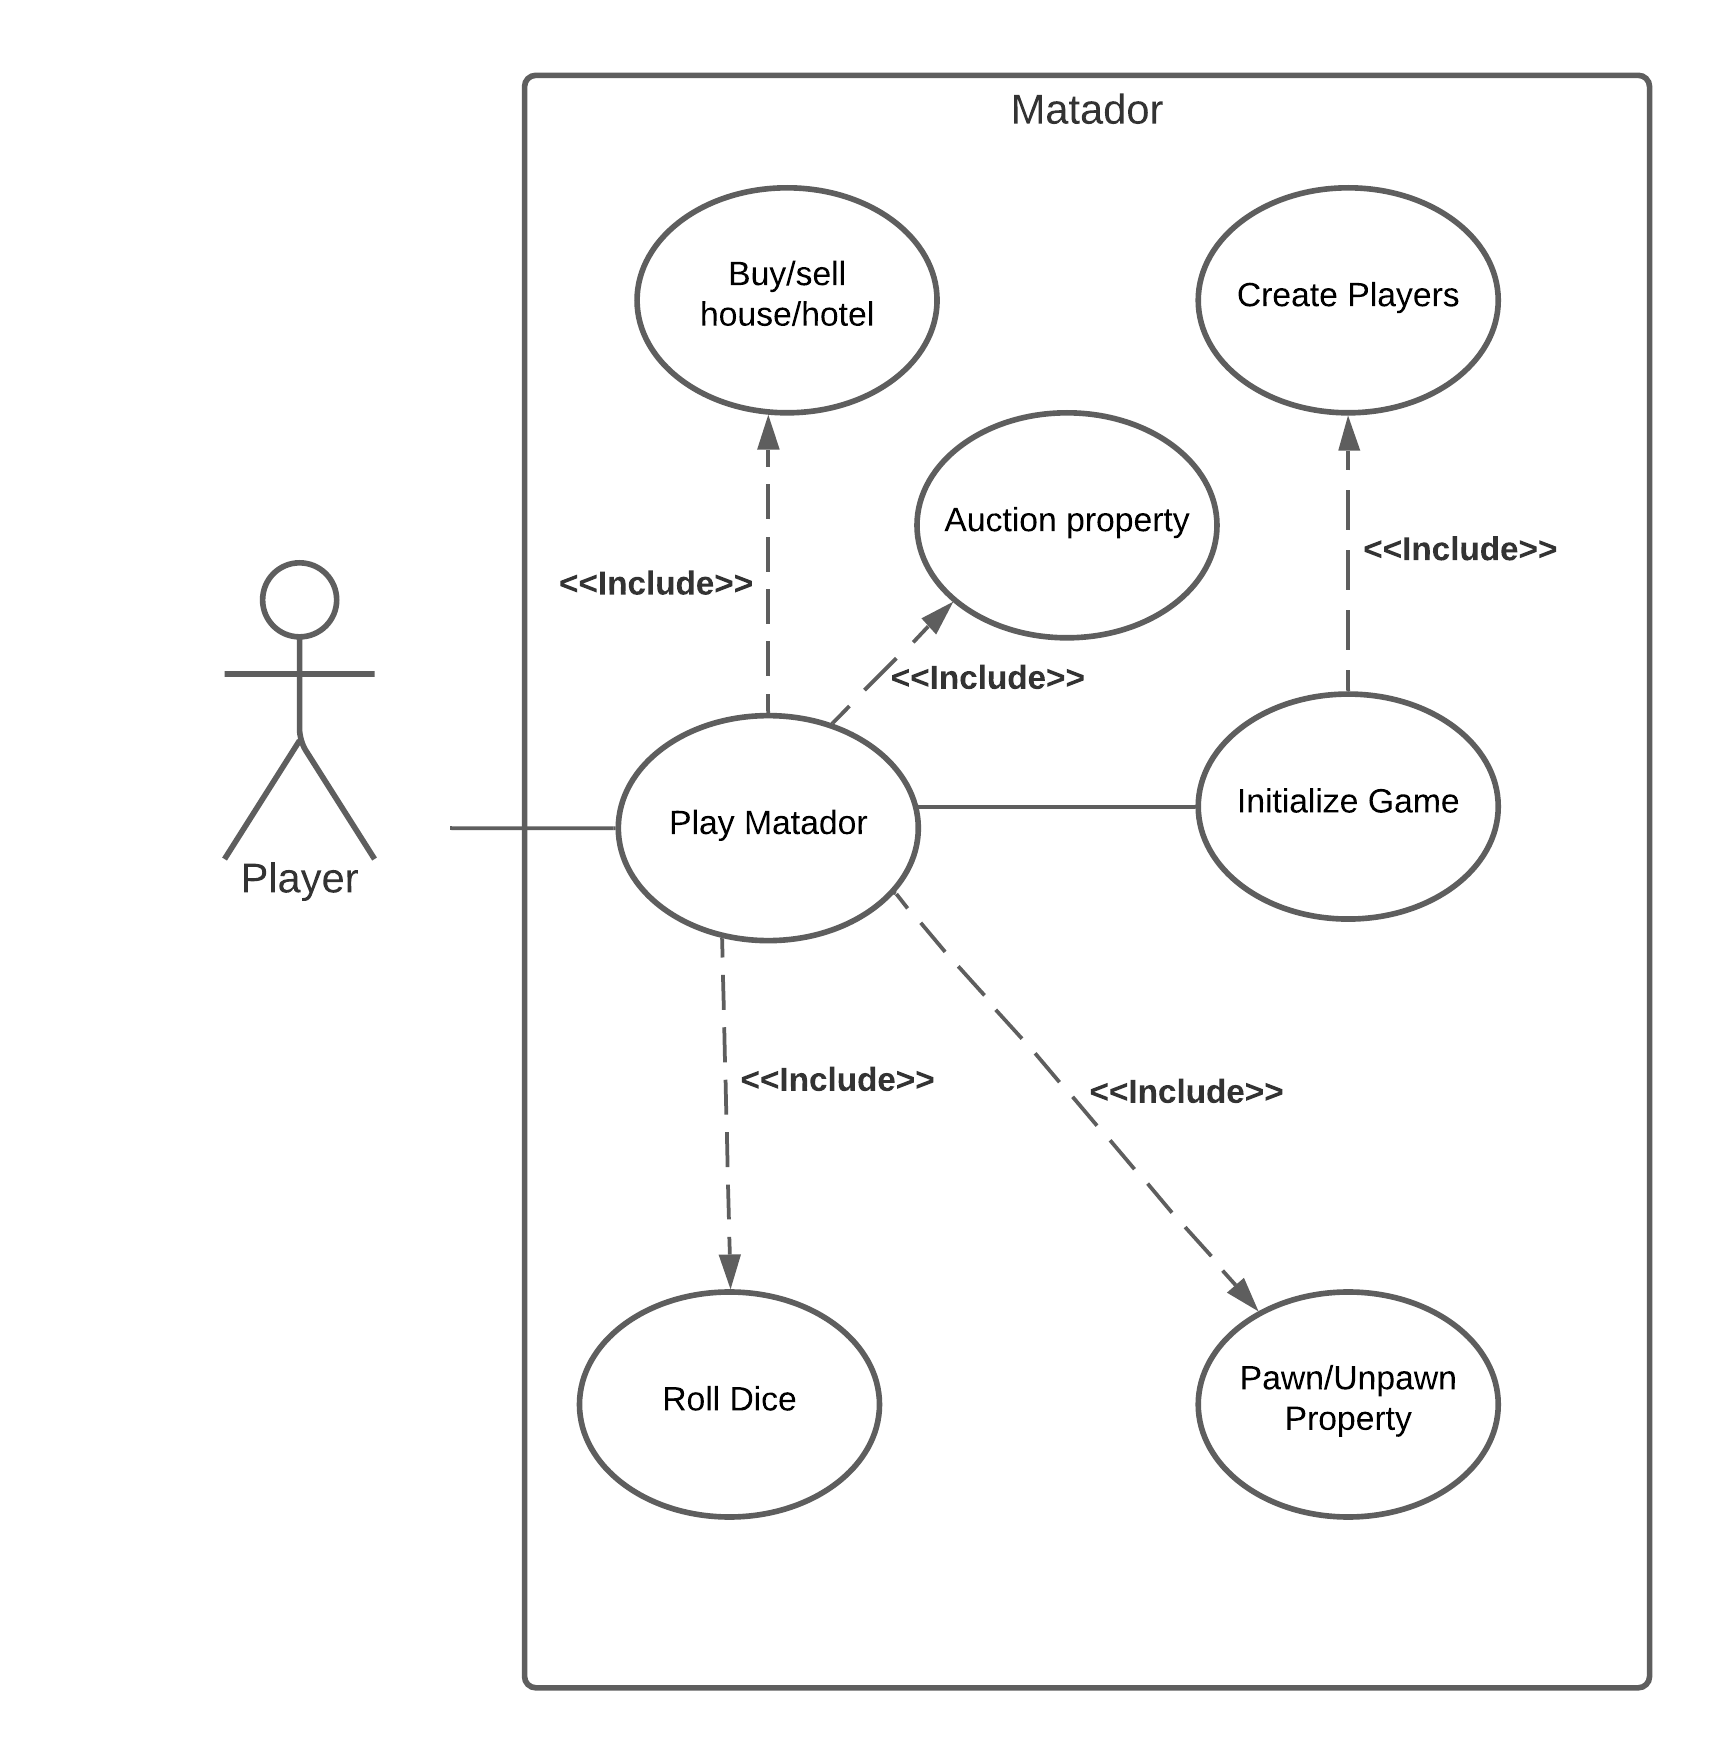
\includegraphics[width=12cm]{Report/figures/Use Case Diagram.png}
    \caption{Use-case diagram}
    \label{use-case diagram}
\end{figure}

\subsection{Central use-case}
Under analysefasen har vi bestemt UC01: Roll dice til at være mest central for Matadorspillet. Derfor har vi udarbejdet en use-case beskrivelse i fully dressed format (se Figure \ref{fully-dressed}. \\

\begin{figure}[htp]
    \centering
\begin{tabular}{ |c|c|c|c|c|c|  }
\hline
\multicolumn{2}{|c|}{Fully dressed use-case} \\
\hline
Use-case section & Comment \\
\hline
Use-case Name & UC01: Roll dice\\
\hline
Scope & Matador Game\\
\hline
Level & User Goal\\
\hline
Stakeholders and Interests & Players\\
\hline
Preconditions & Player chooses the GUI option to roll dice.\\
\hline
Postconditions & Game changes to next player.\\
\hline
Main success scenario & 1. Player rolls dice.\\
                      & 2. Dice values are shown on the GUI.\\
                    & 3. Player object moves on the GUI gameboard\\
                    & according to the sum of dice facevalue.\\
                    & 4. The gameboard field landed on \\
                    & executes its corresponding actions.\\
                    & 5. Current player's turn ends.\\
                    & 6. Game changes to next player.\\
\hline
Extensions & 6a. One player wins the game. \\
                   & 1. Winner is displayed.\\
                   & 2. Game exits.       \\
                   & 6b. A player rolls identical dices. \\
                   & 1. Steps 2 through 4 in Main success scenario\\
                   & are executed, but player can roll dice again. \\
                   & 1a. Player rolls identical dices thrice in a row.\\
                   & 1. Player moves to jail field on gameboard. \\
                   & 2. Continues from step 5 in Main success scenario.\\
\hline
Special Requirements & Arbitrary.\\
\hline
Technology and Data Variations list & N/A.\\
\hline
Frequency of Occurrence & Continuous.\\
\hline
Misc. & N/A.\\
\hline

    \end{tabular}\\
    \caption{Fully dressed use-case af roll dice use-case.}
    \label{fully-dressed}
\end{figure}
\doublespacing

\subsection{Brief use-case beskrivelser}
\textbf{UC02: Play Matador} \\
Her spilles spillet, hvor hver spiller tager deres tur indtil en vinder findes.  \\
\textbf{UC03: Initialize Game} \\
Når initialize Game eksekveres af brugeren, skal der vælges antal spillere, spilleres navne og hvem der starter. Herefter påbegyndes det aktuelle Matadorspil.\\
\textbf{UC04: Buy/sell house/hotel} \\
Når det er en spillers tur kan spilleren vælge at købe og sælge huse hoteller på grunde, som er ejede. Herefter opdateres GUIen og tilføjer eller fjerner huse/hoteller fra grænsefladen.\\
\textbf{UC05: Create Players} \\
Når et spil initialiseres vises der en menu, hvor brugeren kan vælge antal spillere, navngive spillerne og vælge hvem der starter.\\
\textbf{UC06: Auction property} \\
En spiller kan vælge at sætte en grund på auktion. Herved får alle spillere mulighed for at byde i auktionen.\\
\textbf{UC07: Pawn/Unpawn property} \\
En spiller kan vælge at pantsætte eller tilbagekøbe pantsatte grunde. Når en spiller har tilbagekøbt eller pantsat opdateres GUIen med spillerens nuværende konto og grunde, hvortil de pantsatte grunde får en stiplet linje.

\subsection{Domæne model}
For bedre at forstå domænet, der arbejdes i, har vi udarbejdet en domæne model (se Figure \ref{Domænemodel}). I domænemodellen ses en oversigt af de forskellige virkelige objekter, som eksisterer i Matador domænet.
\begin{figure}[H]
    \centering
    \includegraphics[width=16cm]{Report/figures/Domæne model.png}
    \caption{Domæne model}
    \label{Domænemodel}
\end{figure}

\subsection{Systemsekvensdiagram}
Her til at afrunde vores analysedel har vi udarbejdet et systemsekvensdiagram over Matador spillet (se figure \ref{Systemsekvensdiagram}). Diagrammet viser, hvordan en bruger (Player) skal interagere med spillet (Matador). Først starter brugeren spillet, hvorefter spillet viser en menu. Herefter skal brugeren indtaste antallet af spillere, hvorefter brugeren indtaster navne for hver spiller, og vælger hvilken spiller der skal starte. Herefter kører matadorspillet i et loop, hvor spillerne skiftes til at tage deres tur (Take turn) og spillet opdaterer (Game updates) indtil der er fundet en vinder. Til sidst vises, hvem der har vundet og spillet ender.
\begin{figure}[htp]
    \centering
    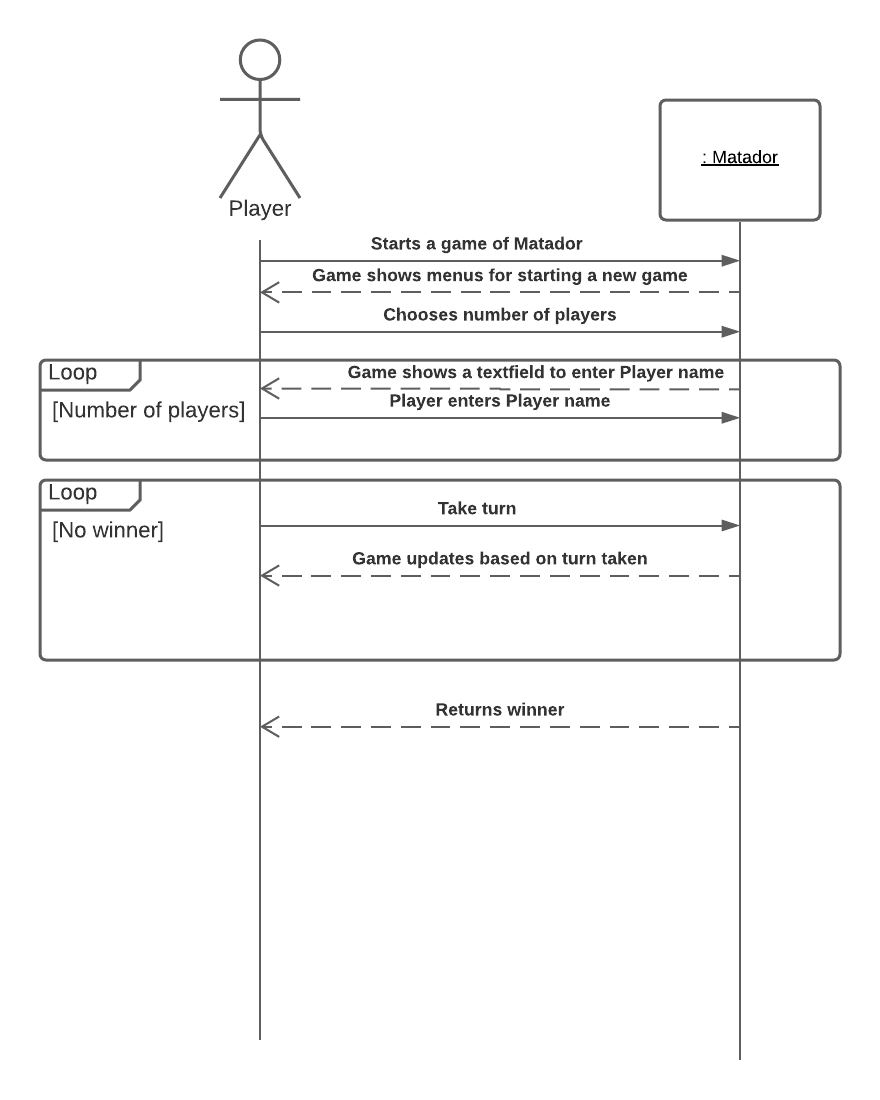
\includegraphics[width=13cm]{Report/figures/System Sekvens Diagram.png}
    \caption{Systemsekvensdiagram}
    \label{Systemsekvensdiagram}
\end{figure}

\end{flushleft}